\section{Tax-Induced Retention and Allocation Gains}\label{sec:framework}\label{sec:welfare}

The policy experiment identifies a response of recorded deeds. Translating
that response into welfare requires two further steps: determining which
properties change allocation, and valuing those changes. This section makes
those steps explicit. Its quantitative results are conditional calibrations
of potential gains from the inheritance provisions, not estimates of
realized gains or the total welfare effect of Proposition~19.

\subsection{Efficient family retention and the tax wedge}

A family allocation can be efficient. An heir may have a strong attachment
to a home, provide housing to relatives, or rent it to a tenant who values
its services highly. None of these uses requires a market sale. Legal title,
occupancy, rental provision, and allocation are therefore distinct objects.

Consider a price-taking household under quasi-linear preferences, with
fixed housing services and no externalities. Let $u_m$ be the annual value
of the house under the alternative market allocation and $u_h$ its value
under family retention, including attachment and the net value of rental
use. These are values of housing services, not recorded deed prices. With
competitive rental markets and no other wedges, the benchmark assumes that
private valuations rank these uses in the same order as social surplus;
rent payments are transfers rather than additional housing services. With
discount rate $r$ and a constant property-tax rate $t$, the benchmark price
is $p=u_m/(r+t)$. A one-time real cost $C$ of switching allocation has
annual equivalent $c=rC$ in this stationary benchmark. Retaining an
inherited assessment $A_0$ is privately optimal when
\begin{equation}
  \frac{u_h-tA_0}{r}\geq p-C
  \quad\Longleftrightarrow\quad
  g\equiv u_m-u_h-c\leq t(p-A_0)\equiv w.
  \label{eq:keep}
\end{equation}
Here $g$ is the annual net resource-surplus gain from changing allocation;
$w$ is the annual tax advantage of retaining the inherited assessment.
Maintaining these assumptions while eliminating the advantage for an
otherwise eligible non-occupant heir changes the threshold from $g\leq w$
to $g\leq0$. Tax-induced inefficient retention occupies the interval
\begin{equation}
  0<g_i\leq w_i,\qquad w_i=t_i(p_i-A_{0i}).\label{eq:distorted}
\end{equation}
When $g_i\leq0$, retaining the house is efficient even without the tax
advantage. A rented home need not have $g_i>0$: changing its owner without
improving its use can leave housing-service allocation unchanged.

Equation~\eqref{eq:distorted} concerns the margin on which the advantage is
fully removed. Proposition~19 retains an exclusion for qualifying
owner-occupants and family farms; the framework does not treat all family
deeds as eligible parent--child successions or assume that all heirs face
full removal. Nor does it model the reform's assessment-portability arm.
Transaction costs and attachment enter $g$, rather than being counted as
additional gains from inducing sales.

\subsection{What the reduced-form response does and does not identify}

The baseline-scaled net-DiD response is
\begin{equation}
 F=\overline D_{\mathrm{CA},2018:2019}
       \left[1-\exp(\widehat\beta_{\rm family}-\widehat\beta_{\rm market})\right]
   =\WelfareFlow\ \text{deeds per year}.\label{eq:flow}
\end{equation}
The baseline is \WelfareBaseline\ deeds; the implied decline is
\WelfareNetPercent\ percent. This is a scaling of a log specification by
a historical baseline, not an independently estimated count of released
houses. Its state-placebo $p$-value is 0.176. The raw and population-adjusted
SCM gaps describe different specifications; their approximately 27--33
percent range is neither a confidence interval nor the input to
equation~\eqref{eq:flow}.

A missing deed can represent postponed paperwork, a different legal
vehicle, or a changed allocation. The null estate-sale evidence does not
identify which explanation dominates. Let $\alpha$ be the number of
distinct, allocation-changing properties per missing deed. We evaluate
$\alpha\in\{0,0.25,0.5,0.75,1\}$ without selecting an empirically preferred
value. This conversion incorporates repeated deeds, title-only responses,
eligibility, and actual use changes. Restricting it to $[0,1]$ assumes at
most one directly affected property per missing deed and excludes indirect
market effects. It is a scenario restriction, not an identified bound on
the reform's total response. The national ratio of 1.19 deeds per parcel
cannot estimate this conversion for marginal California properties.

\subsection{Valuing an allocation change}

Conditional on a common wedge $w$ and a uniform distribution of $g$ among
switchers on $(0,w]$, the mean annual surplus gain is
\begin{equation}
 E[g\mid\text{allocation switcher},w]
   =\frac{1}{w}\int_0^w g\,dg=\frac{w}{2}.
 \label{eq:triangle}
\end{equation}
This is the Harberger-triangle benchmark. More generally write the mean
gain as $\lambda w$. We report $\lambda=0.25,0.5,0.75$; the conditional
support restriction is $0\leq\lambda\leq1$. Uniformity across the entire
removed wedge is an assumption about a finite reform, not a consequence of
deadline bunching. Sufficient-statistics reasoning reduces the required
structure but does not remove the need to justify the mapping from
behavior to welfare \citep{chetty2009sufficient}.

For heterogeneous properties the relevant object is the survivor-weighted
sum of $g_i$, not the product of an unconditional average wedge and an
average survival rate. Our separable benchmark holds the annual wedge and
mean gain fixed and uses a common persistence profile. Sensitivities vary
each component; they do not identify the joint distribution of wedge,
valuation gap, and duration.

We use an external wedge benchmark because deed prices do not value unsold
homes and the available property-characteristics snapshot does not identify
the pre-reform assessment gap of marginal heirs. The LAO reports a
\$3,000--\$4,000 annual tax saving for a long-held Los Angeles home
\citep{lao2017inheritance}. Treating the unspecified dollar vintage as the
2017 publication year and using annual CPI-U gives an inflation factor of
\WelfareInflator: a \$\WelfareWedgeLow--\$\WelfareWedgeHigh\ range and a
\$\WelfareWedge\ midpoint in 2023 dollars \citep{bls2023cpi}.
This is a location- and tenure-specific benchmark, not a measured statewide
marginal wedge. Appendix~\ref{app:welfare} reports the valuation audit and
half/double-midpoint stress cases.

\begin{table}[!ht]\centering
\caption{Inputs to the welfare calibration}\label{tab:welfare_inputs}
{\small
\begin{tabular}{p{0.22\textwidth}p{0.25\textwidth}p{0.42\textwidth}}\toprule
Input & Value & Evidence status \\
\midrule
Recorded-deed flow & 58,045 per year & Net DiD scaled by 2018--2019 CA baseline \\
Net DiD inference & $p=0.176$ & State placebo rank; not a welfare test \\
Annual tax wedge & \$3,729--\$4,972 & LAO long-held Los Angeles benchmark \\
Source dollar year & 2017 & Assumed publication-year dollars; CPI to 2023 \\
Allocation conversion & $\alpha\in[0,1]$ & Assumed properties per missing deed \\
Mean surplus gap & $\lambda w$ & Uniform benchmark $\lambda=1/2$ \\
Persistence & CA parcel-episode survival & Proxy; marginal survival is not identified \\
Delay / horizon & 0, 5, 10 / 10 years & Assumptions; grandfathered stock excluded \\
\bottomrule\end{tabular}}
\begin{minipage}{0.96\textwidth}\vspace{3pt}{\scriptsize\textit{Notes:} The tax wedge is an external benchmark, not a statewide marginal estimate. The SCM estimates are reported separately and do not enter the net-DiD reference flow. The conversion parameter includes legal-title-only responses and multiple deeds per property; it is not estimated using the national deeds-per-parcel ratio.}\end{minipage}\end{table}


\subsection{From a flow of deeds to potential property-years of gain}

Let $S(a)$ describe how long the counterfactual allocation loss persists
after succession, and let $L$ be the delay between a missing deed and that
succession. For a cohort $c$, use $F_c=F$ as an explicit constant-flow
extrapolation. The potential stock of avoided misallocation at year $T$ is
\begin{equation}
 N_T(\alpha,L)=\sum_{c=2022}^{T}\alpha F_c
   \mathbf1\{T-c\geq L\}S(T-c-L),\qquad
 G_T=\lambda wN_T.\label{eq:stock}
\end{equation}
The illustration runs from 2022 through 2031. It starts with no inherited
stock of reform gains: transfers already protected under Proposition~58
were not retroactively reassessed \citep{boe2025prop19}. Anticipatory deeds
completed under the old rules are not newly treated cohorts. Continuing
the 2022--2023 response for a decade is a policy scenario, not a forecast.

For persistence we construct California parcel episodes beginning in
2008--2018. An episode begins at the first qualifying family deed since the
previous market sale and ends at the next market sale or the June 30, 2024
censor. Further family deeds within the episode do not create additional
houses. Ten-year survival is \WelfareCABroadSurvival\ percent for broad
family episodes and \WelfareCASameSurvival\ percent for same-surname
episodes. These are descriptive proxies for persistence, not survival
estimates for the unobserved marginal homes. A home can remain unsold while
its use improves; conversely, an allocation loss need not end exactly at
sale. Appendix sensitivities use both episode definitions and multiply
cumulative hazards by one-half and two.

\begin{table}[!ht]\centering
\caption{Potential allocation gains: conditional calibration}\label{tab:welfare}
{\small
\begin{tabular}{rrrrrr}\toprule
$\alpha$ & Delay & Stock in 2031 & Property-years & Annual gain & Ten-year PV \\
 & (years) & (thousands) & (thousands) & (\$m, 2031) & (\$m) \\
\midrule
0.00 & 0 & 0.0 & 0.0 & 0.0 & 0.0 \\
0.00 & 5 & 0.0 & 0.0 & 0.0 & 0.0 \\
0.00 & 10 & 0.0 & 0.0 & 0.0 & 0.0 \\
0.25 & 0 & 110.6 & 654.9 & 240.6 & 1,167.0 \\
0.25 & 5 & 62.2 & 194.8 & 135.3 & 328.7 \\
0.25 & 10 & 0.0 & 0.0 & 0.0 & 0.0 \\
0.50 & 0 & 221.2 & 1,309.7 & 481.2 & 2,334.1 \\
0.50 & 5 & 124.4 & 389.5 & 270.6 & 657.4 \\
0.50 & 10 & 0.0 & 0.0 & 0.0 & 0.0 \\
0.75 & 0 & 331.8 & 1,964.6 & 721.7 & 3,501.1 \\
0.75 & 5 & 186.6 & 584.3 & 405.9 & 986.1 \\
0.75 & 10 & 0.0 & 0.0 & 0.0 & 0.0 \\
1.00 & 0 & 442.4 & 2,619.5 & 962.3 & 4,668.2 \\
1.00 & 5 & 248.8 & 779.1 & 541.1 & 1,314.8 \\
1.00 & 10 & 0.0 & 0.0 & 0.0 & 0.0 \\
\bottomrule\end{tabular}}
\begin{minipage}{0.96\textwidth}\vspace{3pt}{\scriptsize\textit{Notes:} All dollars are 2023 dollars. The assumed annual wedge is the CPI-adjusted LAO midpoint; $\lambda=1/2$, the real discount rate is 3\%, and persistence uses California broad-family parcel episodes. Cohorts enter annually in 2022--2031. No value of $\alpha$ is empirically preferred. Rows are scenarios, not confidence intervals; zero response and ten-year delay give zero gains within the horizon.}\end{minipage}\end{table}


Table~\ref{tab:welfare} displays how strongly the answer depends on the
unidentified conversion and delay. For illustration, $\alpha=0.5$ and a
five-year delay imply \WelfareExampleStock\ potentially affected properties
in 2031, an annual gain of \$\WelfareExampleAnnual\ million in that year,
and a discounted ten-year gain of \$\WelfareExamplePV\ million. These
numbers use the midpoint wedge, $\lambda=1/2$, and a 3 percent real discount
rate. They are not preferred estimates. With $\alpha=0$, every missing deed
is consistent with zero allocation gain; with a ten-year delay, no gains
occur inside the reporting horizon. No positive welfare lower bound follows
from the reduced-form estimates.

\begin{figure}[!ht]\centering
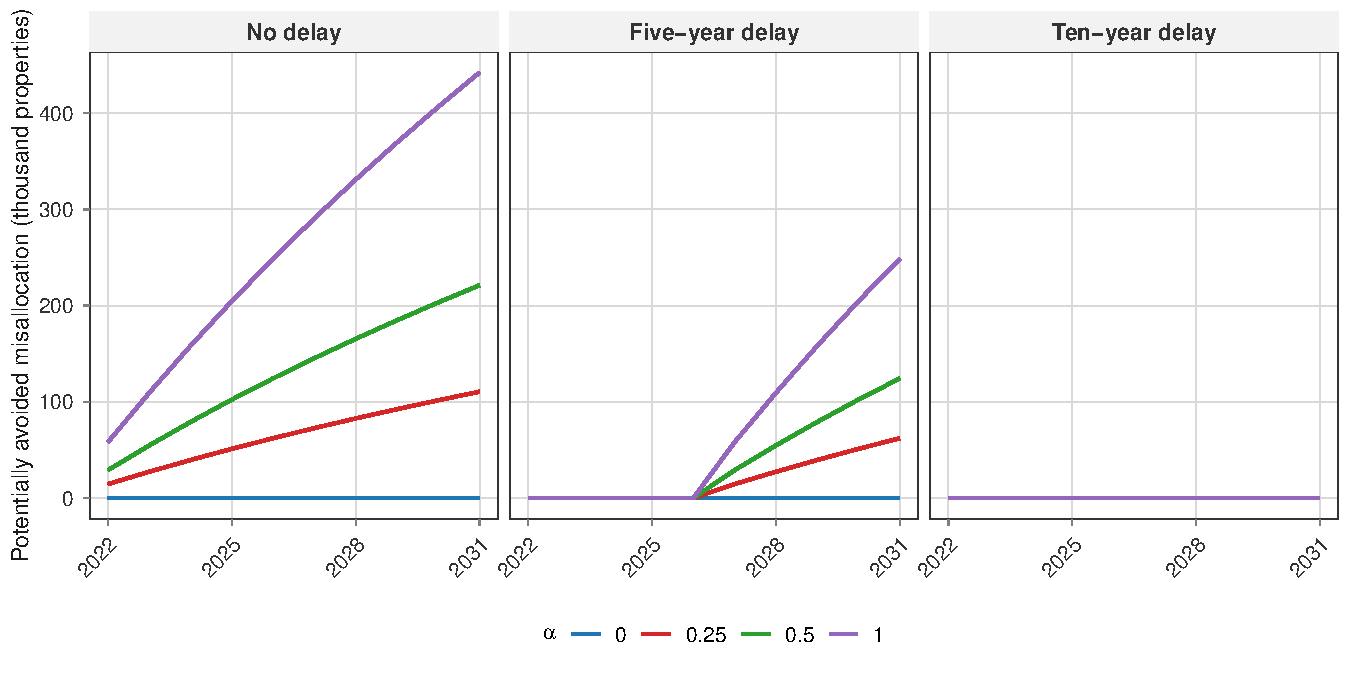
\includegraphics[width=0.98\linewidth]{figures/F8_welfare_stock.pdf}
\caption{Potential stock of avoided misallocation under alternative conversion
rates and succession delays. All paths assume a constant annual reference
flow and California broad-family episode persistence. These are conditional
scenarios, not observed stocks or forecasts.}
\label{fig:welfare_stock}
\end{figure}

\subsection{Incidence and the limits of the policy calculation}

Removing an inheritance exclusion can raise an heir's taxes and government
receipts even when housing use does not change. With equal welfare weights
and a dollar-for-dollar budget offset, these payments cancel in aggregate;
they are not resource gains. Inframarginal heirs can bear substantial tax
increases while contributing zero to $G_T$. Buyers and tenants gain only
to the extent that housing is allocated to a more valuable use after
accounting for attachment, displacement, and real switching costs.

The ledger in Appendix~\ref{app:welfare} separates these components. We do
not estimate public-spending benefits, marginal costs of public funds,
distributional welfare weights, general-equilibrium prices or rents, or
gains from expanded assessment portability. Accordingly, this exercise
quantifies a potential allocation component of the inheritance reform,
conditional on the reduced-form interpretation and additional assumptions.
It neither measures total Proposition~19 welfare nor extrapolates
California's tax wedge to the national family-transfer channel.
